\chapter{研究智能体大语言模型的行为}\label{chap:behavior}

\begin{learningbox}
本章将介绍智能体大语言模型的行为与人类行为有何异同。
具体而言，学完本章后，你将能够：
\begin{itemize}[leftmargin=*, nosep]
    \item 解释{\em 大语言模型行为}的含义，并描述如何研究这种行为。
    \item 列举{\em 基本的社会与交互能力}，说明大语言模型在哪些方面表现良好，在哪些方面仍然存在困难。
    \item 描述研究大语言模型高级社会与交互能力的方法，尤其是{\em 策略思考}、{\em 心智理论}与{\em 道德推理}。
    \item 结合{\em 测试与解释}中的各种问题，反思研究大语言模型的行为方法能够和不能够告诉我们什么。
\end{itemize}
\end{learningbox}

\section{什么是大语言模型行为？}
2019 年，一个由计算科学、行为科学和认知科学研究者组成的团队，描述了一个新研究领域的兴起：\emph{机器行为（machine behavior）}。这一领域旨在{\em 对智能机器开展科学研究，将其视为一类具有特定行为模式和生态关系的行动者，而不仅仅是工程产物} \citep{rahwan_machine_2019}。机器行为研究本质上具有跨学科性质，因为它将{\em 技术}内部层面的知识，即算法、数据结构与训练过程，与其实际使用时的\emph{环境和情境}知识整合起来。

机器行为研究的方法可与动物行为学或心理学的工作相比：在这些领域，要进一步理解动物和人的运作方式，同样需要整合内部层面，例如生物物理学、神经学，以及生态层面，即与环境的交互、社会交互，所提供的认识。

本部引言已经提到研究机器行为，尤其是大语言模型行为的一个重要现实动机：随着大语言模型越来越多地融入我们的日常工作和个人生活环境，认识并理解它们的行为倾向与模式已经成为紧迫的任务。

这也有科学上的动机：由于大规模神经网络架构十分复杂，它们看起来如同{\em 黑箱}，因此很难通过解析方法追溯其运作过程。（不过，机制可解释性领域确实在尝试这样做，见第~\ref{chap:mi}~章。）通过实证方法研究这类复杂系统的{\em 行为}，是增进理解的一条互补路径。换言之，由于交互的复杂性，即使一位理论上的工程师掌握了某个大语言模型架构和训练数据的全部知识，仍可能无法预测它在不同情境中会如何回应。行为研究方法旨在填补这一空白。

什么可以算作\emph{行为}，取决于被研究系统的可供性（affordance）\footnote{{\em 可供性}指系统在特定情境中，基于其设计与实现方式所能做的事情。}以及研究范围。例如，对一个基础大语言模型而言，行为就是模型基于词元的推理所产生的{\em 输出}。另一方面，对于能够进行网页搜索、运行代码等操作的智能体大语言模型，行为还可以包括它为得到某种输出或实现某种效果而执行的{\em 动作}。我们将看到，一些研究仅考虑最终输出，并将其视为模型的行为；另一些研究也关注中间步骤。

\section{通过实验探查大语言模型行为}
近年来，出现了许多测试大语言模型社会与交互能力的研究。主要有两种方法：(1) 将原本为人类开发的实验范式改编为测试项目，用来提示模型；(2) 专门为大语言模型开发新的测试范式。后一种方法既可以采用大规模基准测试进行定量研究，也可以在较小规模上进行深入的人工分析，开展定性研究。下文将介绍相关例子。

将行为学与心理学方法用于大语言模型，包括智能体大语言模型，并非简单直接的事情。为人类设计的实验假定受试者是具身主体，具有信念、愿望，以及在时间上持续存在的自我感。智能体大语言模型并不以任何显而易见的方式具备这些特征。这就要求我们反思\emph{构念效度（construct validity）}：测量人工智能系统中的某种特质或能力，究竟意味着什么？这一问题涉及两个层面：某种特质的可观测结果，以及产生结果的底层机制。第~\ref{sec:theoryofmind}~节将讨论{\em 错误信念测试（false-belief test）} \citep{carpenter2002new}这一例子。虽然研究已经表明，一些类别的模型在回答这类测试问题时与人类相似，即在行为结果层面相似，但在 Transformer 模型与人类中，产生这种行为的底层机制有多大程度的差异或重合，目前仍不清楚。第~\ref{chap:cognition}~章将更深入地讨论构念效度问题。

对于大语言模型专用测试，也需要考虑方法上的挑战。例如，已知大语言模型对提示中看似无关的变化，如词序、逗号等，可能高度敏感；它们也可能由于采样变异、模型温度或随机种子不同，在多次运行中产生不同输出。此外，实验材料泄漏到训练数据中，可能使模型的表现建立在记忆而非泛化之上。接下来几节将介绍若干具体例子。本部各章末尾都会关注方法的严谨性与解释时应有的审慎。

下面几节首先讨论智能体交互所需的基本社会能力。随后，我们考察智能体围绕其他智能体行为进行推理的策略行为，并讨论心智理论。最后，我们讨论大语言模型的道德判断。

\section{基本社会能力工具箱}
本节概述基本的社会与交互能力，包括对话、语用与社交礼仪。

\subsection{功能语言能力与语用能力}
如第一部所述，经过指令微调的大语言模型，其关键进步是能够像聊天机器人一样使用自然语言进行交互。这不仅要求一定程度的\emph{形式语言能力（formal linguistic competence）}，即生成正确、合乎语法的句子，还要求\emph{功能语言能力（functional linguistic competence）}，即在特定语境中理解话语含义的能力 \citep{mahowald2023dissociating}。在语言学与认知科学中，功能语言能力是{\em 语用学（pragmatics）}的研究对象。语用学的核心概念可以追溯到 20 世纪中叶语言哲学的{\em 语用转向（pragmatic turn）}：语言意义在很大程度上并非内在于符号本身，如词元、词语和句子，而是在于它们在实际语境中的使用。这既包括\emph{语言语境（linguistic context）}，其范围从周围词语延伸到标题、体裁等较远因素，也包括\emph{非语言语境（extra-linguistic context）}，涵盖空间、时间和社会维度。这种观点最著名的表述是 Paul Grice 的\emph{会话含意（conversational implicature）}概念 \citep{Grice_1975}。请看以下例子：

\begin{enumerate}
    \item A：请问，你能把盐递给我吗？B：能。你还希望我真的递给你吗？
    \item A：Sarah 是个好同事吗？B：嗯，这么说吧，她总是很准时。
    \item 他发出了一连串声音，与一首咏叹调的乐谱相当吻合。
\end{enumerate}
Grice 认为，语言使用受到\emph{合作原则（cooperative principle）}的支配：我们假定交谈对象，无论是人类还是智能体，都在尝试进行有意义的交流。上例 1 中，B 破坏合作原则的做法是一个经典例子：询问你能否递盐的人，通常并不是想得到一个确认这种可能性的字面回答，而是希望你实际把盐递过来。在例 2 中，B 的回答明显只聚焦于一个狭窄方面，即守时，听者可以由此推理出，例如，B 在暗示 Sarah 在同事相处方面存在不足。同样，当某人说出例 3，而不是简单地说{\em 他唱了一首咏叹调}时，过分繁复的措辞可能暗示其对这次表演的某种态度，例如说话者并不喜欢这次表演。在这些例子中，字面所说的都只是信息的一部分；另一部分则需要听者根据语境解读，或者说{\em 领会言外之意}。

以灵活、依赖语境的方式理解语言意义，长期以来都是自然语言处理中的一个著名难题 \citep{trott-etal-2020-construing}。人们普遍认同，大语言模型在这一问题上取得了重大进展，但对造成这些进展的因素仍缺乏充分理解。模型规模是功能语言能力与语用能力的重要预测因素，某些微调方式，尤其是监督微调（SFT）和直接偏好优化（DPO），也是如此 \citep{yu-etal-2026-pragmatic, ruis2023goldilocks}。然而，大语言模型在不同功能理解与语用理解领域中的表现差异仍然很大，总体得分也远低于人类 \citep{sravanthi2024-pub}。

一种解释是，大语言模型能够获取的非语言语境信息较少：它们无法像与之交互的人类一样看、听或以其他方式感知，而且在大多数情况下，它们并不了解此前的交互 \citep{vandermeulen2025properly}。随着模型转向智能体大语言模型，这一状况可能正在改变，因为模型开始配备记忆、多模态能力，以及其他能够补充语境的工具。目前仍缺乏关于这些变化如何影响表现的实证数据。

\subsection{礼貌与社交礼仪}
人机交互中的社交礼仪与礼貌，已有数十年的研究历史 \citep{ribino2023role}。一个有用的理论基础是\emph{计算机是社会行动者（Computers Are Social Actors，CASA）}范式 \citep{nass1994computers}。它认为，即使我们知道机器并非人类社会行动者，仍倾向于将人类常用的社会规则与期望应用于计算机。我们通过表达礼貌、个性与互惠的线索，并对这些线索作出回应，来与机器建立和调整信任与接受关系。研究表明，机器遵守社交礼仪时，人类会更加信任它们 \citep{miller2005}，任务表现与用户满意度也会随之提高 \citep{miyamoto2021}。下面讨论礼貌理论及其在大语言模型中的应用。

\paragraph{礼貌理论}
经典礼貌理论 \citep[例如][]{brown1987politeness}直接建立在上述 Grice 的观点之上。这一理论认为，交谈者一直在维护彼此的\emph{面子（face）}，即每位参与者都希望维持的公共自我形象。面子有积极维度，即希望得到他人的喜爱与认可，也有消极维度，即希望避免社会阻碍。从 Grice 的视角看，许多日常请求、批评与拒绝本身就是\emph{威胁面子的行为（face-threatening act）}，说话者因此会采用礼貌策略应对。这个框架为大语言模型研究者提供了一套术语，用以考察大语言模型及其用户能否识别面子威胁，并以适合语境的方式缓解这些威胁。

\paragraph{大语言模型对用户有礼貌吗？}
一个相关研究方向是，模型自身所表现的礼仪是否符合社会与文化要求。上一小节指出的局限在这里再次出现：大语言模型能够获取的非语言语境信息很贫乏。礼貌具有文化特异性，但主要使用英语数据训练的系统往往默认采用英语文化中偏重直接表达的规范 \citep{havaldar2023comparing}。关于波斯语 \emph{taarof} 的研究清楚地展示了这一问题。taarof 是一套仪式化的提议与推辞体系，其中恰当的回应往往与直接回应相反。一项研究表明，在文化上应当遵循 taarof 的情境中，前沿模型的表现比母语者低 40\% 以上，反而默认采用西方式的直接表达。这导致了表面礼貌与文化适切性之间的脱节。例如，在一项研究中，按标准指标判断，所研究模型的回答有 84.5\% 被评为{\em 有礼貌}，但只有 41.7\% 被判定为符合文化要求 \citep{goharisadr2025taarof}。在西方礼貌评分标准中取得高分，并不等于在所有情境中都表现得恰当。这提醒我们，在测量模型的礼貌程度时，需要持续反思构念效度。

\paragraph{用户的礼貌程度会影响大语言模型的表现吗？} \label{sec:politeness}
一项涵盖英语、汉语和日语任务的研究发现，不礼貌的提示往往会降低多种模型的表现 \citep{yin-etal-2024-respect}。研究还发现，过度礼貌并没有带来可靠收益，而且最佳礼貌程度随语言和文化背景而变化。这一结果符合“计算机是社会行动者”范式：大语言模型似乎从训练数据中再现了人类将粗鲁与合作失败联系起来的倾向。然而，\citet{dobariya2025tone} 报告了一个直接相反的结果：在一个多项选择基准测试中，对于 GPT-4o，直白甚至粗鲁的提示比礼貌提示的表现略\emph{好}。因此，语气与质量之间的对应关系似乎既不在不同代际模型中保持稳定，也不简单明了。这体现了本章前面提出的提示敏感性与可复现性问题，也提醒我们，不应将任何单一的语气效应视为大语言模型本身的稳健属性。

综合来看，大语言模型能够再现礼貌的表面标记，而且确实对交谈者的礼貌程度敏感；但它们既不能以跨文化的稳健方式应用这些规范，也没有表现出语气与任务表现之间的稳定关系。

需要记住的是，迄今的研究仅将礼貌与礼仪限定在交互的语言维度。这与人际交互的多维性形成对照，后者还涉及面部表情、手势和其他情境线索 \citep{brown1987politeness}。与语用能力类似，转向配备记忆、能够更多获取用户特定情境的多模态智能体大语言模型，有望改善对特定用户规范的适应，但目前实证证据仍然很少。

\subsection{对情绪与情感线索的敏感性} \label{sec:empathy}
胜任社会交互，不仅需要理解话语的含义，即语用，还需要以有效、恰当的方式表达，即礼仪，也需要对交互中的\emph{情绪与情感}维度保持敏感。这要求识别交谈者的感受，并作出符合对方情绪状态、让对方感到恰当的回应。对人类而言，这种能力与\emph{情绪智力（emotional intelligence）}密切相关。\citet{salovey1990emotional} 将情绪智力定义为理解自己与他人的情绪信息，并利用这些信息引导思考与行为的能力。随着大语言模型越来越多地部署于辅导、客户服务和心理健康支持等情绪色彩浓厚的场景，它们能否以及如何处理情感信息，已成为一个重要研究方向。

\paragraph{共情与情感的定义}
共情与情感是情绪智力研究的核心概念。\emph{情感（affect）}是涵盖情绪、心境与感受的统称。研究通常根据所体验状态的感受性质，将其沿两个维度操作化：效价（valence，愉快—不愉快）与唤醒度（arousal，平静—兴奋）\citep{russell1980circumplex}。相比之下，\emph{共情（empathy）}是面向他人体验状态的一种关系：识别或分享他人的感受。简言之，情感是第一人称的感受，而共情则从第二人称立场对这种感受作出反应。

\citet{devignemont2006empathic} 的论文进一步将共情定义为涉及这样一种情感状态：(1) 与他人的情感状态一致；(2) 通过观察他人的动作、表情和处境而被引发；(3) 同时意识到，这一状态来源于他人的状态。最后一个条件称为\emph{自他区分（self-other distinction）}，它将共情与\emph{情绪感染（emotional contagion）}区分开来。情绪感染是一种更基础的倾向，即受到他人情感状态的感染并与之产生相同感受，却不一定识别出其来源。

情绪感染在自然界中十分普遍。例如，两只小鼠在灌木丛中觅食时，若其中一只的脚被卡住，它在挣扎脱困时会表现出应激迹象。这种应激往往会传播给同伴，而同伴不一定知道原因 \citep{preston2002empathy}。同样的低层机制也存在于认知能力更复杂的物种中，包括我们这样的灵长类动物。不过，自他区分增加了反思的可能性：不仅分享他人的状态，还将其识别为他人的状态，并理解其性质与原因。这进而支持更灵活的回应，例如有针对性的帮助，即采取行动，消除他人痛苦的来源。\footnote{不过，这些层次之间的界限仍是一个活跃的研究课题。例如，大鼠会学会将受困的同笼伙伴从束缚装置中释放出来，甚至为此放弃或分享巧克力奖励 \citep{bartal2011empathy}。作者将其解释为由共情驱动的帮助行为。这类帮助究竟体现了具有自他区分的真正共情，还是由帮助者为减轻自身因情绪感染而产生的痛苦所驱动，目前仍有争论。}

另一种广泛使用的区分是\emph{认知共情（cognitive empathy）}，即理解他人的感受、视角或处境，与\emph{情感共情（affective empathy）}，即在情绪上与该状态共鸣或对其作出回应 \citep{dvash2014theory}。两者由部分不同的系统支持：认知共情与心智理论密切相关，后者指将心理状态归属于他人的能力，见第~\ref{sec:theoryofmind}~节；情感共情则与情绪智力有关 \citep{dvash2014theory, preckel2018interaction}。这一区分对评估很重要，因为一个回答可能准确识别出用户的感受，却没有传达任何温暖；也可能听起来温暖、具有支持性，却没有准确理解情境。因此，大语言模型共情研究越来越多地对这两个维度分别评分。

\paragraph{大语言模型中的共情与情感}
大语言模型是否{\em 具有共情能力}，可以有两种理解。我们可以问，它是否像人类或其他动物一样{\em 感受到}某些东西；这是一个复杂问题，这里暂且搁置，留到第~\ref{chap:cognition}~章讨论。另一种理解是考察\emph{感知共情（perceived empathy）}：用户在多大程度上感到大语言模型的回答能够体察情绪并提供支持。一个模型即使纯粹作为文本预测系统运行，也可以生成让人读来感到关怀的语言 \citep{sorin2024large}。明确保持这一区分，再次体现了贯穿本章的构念效度警示：不应将可观测行为，即读起来具有共情的回答，与一种可能存在也可能不存在的底层机制，即实际感受到的情绪状态，混为一谈。

在识别方面，大语言模型能够辨认文本中细粒度的情感与情绪状态 \citep{broekens2023fine}，并将这些信息纳入回应，生成在对话中起到更强共情作用的输出 \citep{yang2024enhancing, yan2024talkhumanlikeagentsempathetic}。这一领域的基准测试之一是 EmpatheticDialogues \citep{rashkin2019towards}。

在表达方面，对于日常情绪情境，人类评分者往往认为大语言模型的回答比人类撰写的回答更具共情，尽管同样的输出也可能呈现出明显的程式化模式，例如反复出现的措辞、特征性的标点和表情符号使用方式 \citep{lee2024large}。

为了测量书面文本中表达出来的共情，一些研究采用 EPITOME 框架 \citep{sharma2020computational}，从三种机制对回答进行编码：\emph{情绪反应}，即温暖、关切与关怀；\emph{理解表达}，即传达出对他人正在经历之事的理解；以及\emph{探索询问}，即通过提问来了解更多。情绪反应对应情感共情，理解表达对应认知共情，因此，这个框架便于将上述概念区分与具体的回答评分联系起来。

一个反复出现的发现是，大语言模型在这两个共情维度上的表现并不均衡。\citet{yu2025can} 使用标准化心理测量工具，报告 GPT-4 再现了在人类身上观察到的认知—情感共情结构，不过总体水平较低；而一个 Llama-3 模型并未表现出同样与人类一致的结构。\citet{williams2025heartificial} 同样发现，无论规模较小还是较大的语言模型，在认知共情任务上都表现出色，但情感共情弱于人类参与者。这一暂时形成的图景，即认知共情强于情感共情，是符合直觉的：认知共情依赖心理状态推理，而大语言模型已经表现出这方面的能力，见第~\ref{sec:theoryofmind}~节；情感共情则意味着某种更接近真实感受的东西。

这里有三点需要注意。第一，用来比较的工具是为人类设计的，只经过了表面调整便用于测试大语言模型。第二，方法仍不一致：\citet{sorin2024large} 的系统综述发现，大多数早期研究集中于医疗情境中的少数模型，并依赖主观的人类判断；该综述还指出了一些混杂因素，例如不论内容如何，\emph{较长}的回答都更容易被评为更具共情。第三，与语用和礼貌研究一样，迄今研究的共情几乎完全局限于文本，剥离了人类交互中承载大量情感信息的声音、面部和身体线索。对于传统大语言模型，这里考察的能力也仅限于即时对话语境。人们普遍预期，转向配备持久记忆、用户特定情境与多模态输入的智能体大语言模型，将增强情感敏感性与个性化 \citep{sravanthi2024-pub}；但与前面几个小节一样，目前直接实证证据仍然稀少。

\subsection{小结}
当前大语言模型在若干基本社会与交互能力上取得了令人印象深刻的进展，这些能力长期以来都是人工智能与人机交互的研究对象。研究者已经开发了行为方法，用于考察这些能力的性质与适用性。虽然加入智能体功能进一步增强了大语言模型的社会与交互潜力，但挑战仍然存在；持续反思这些能力的局限，以及研究它们所用方法的局限，十分重要。

\section{策略行为} \label{sec:strategic}
现在转向策略行为研究，即智能体围绕其他智能体的行为进行推理。我们已经看到，智能体的沟通方式深受其试图达成的目标，也就是其意图的影响。博弈论是研究智能体策略行为的领域 \citep{von2007theory}，关注稀缺资源分配、公平性、均衡条件和社会困境等问题 \citep{jones2000game}，并且长期以来一直使用机器学习方法开展这些研究 \citep{fatima2024learning}。最近，研究者开始转向大语言模型，考察它们的行为与其他类型计算架构有何不同，以及其策略行为与人类有何差异。这些研究通常使用未经额外增强的模型，将一份脚本作为提示提供给模型，而没有加入智能体推理扩展，见第~\ref{chap:reasoning}~章，或工具，见第~\ref{chap:tools}~章。

近期文献呈现出两点认识：在奖励自身利益的博弈中，大语言模型表现得出人意料地合作；而在需要协调的博弈中，它们的表现又出人意料地差。下面先回顾这些发现，再转向测试大语言模型泛化能力的系统性基准工作，以及近期有关前沿推理模型的研究；后者从一些重要方面使这一图景变得更为复杂。

\begin{figure}
  \begin{center}
    \begingroup
\linespread{1}\selectfont
\definecolor{chfifteencream}{RGB}{255,239,199}
\definecolor{chfifteenblue}{RGB}{173,210,235}
\definecolor{chfifteencoral}{RGB}{255,143,132}
\definecolor{chfifteencyan}{RGB}{0,174,228}
\definecolor{chfifteengreen}{RGB}{75,117,49}
\definecolor{chfifteengold}{RGB}{182,135,26}
\resizebox{0.99\linewidth}{!}{%
\begin{tikzpicture}[x=0.01cm,y=-0.01cm,
  every node/.style={inner sep=0pt,outer sep=0pt},
  chtext/.style={anchor=north west,align=left,font=\fontsize{7.1pt}{8.1pt}\selectfont},
  chtitle/.style={font=\bfseries\fontsize{9.5pt}{10pt}\selectfont},
  chlabel/.style={font=\bfseries\fontsize{7.8pt}{8.2pt}\selectfont}]
\node[anchor=north west] at (0,0) {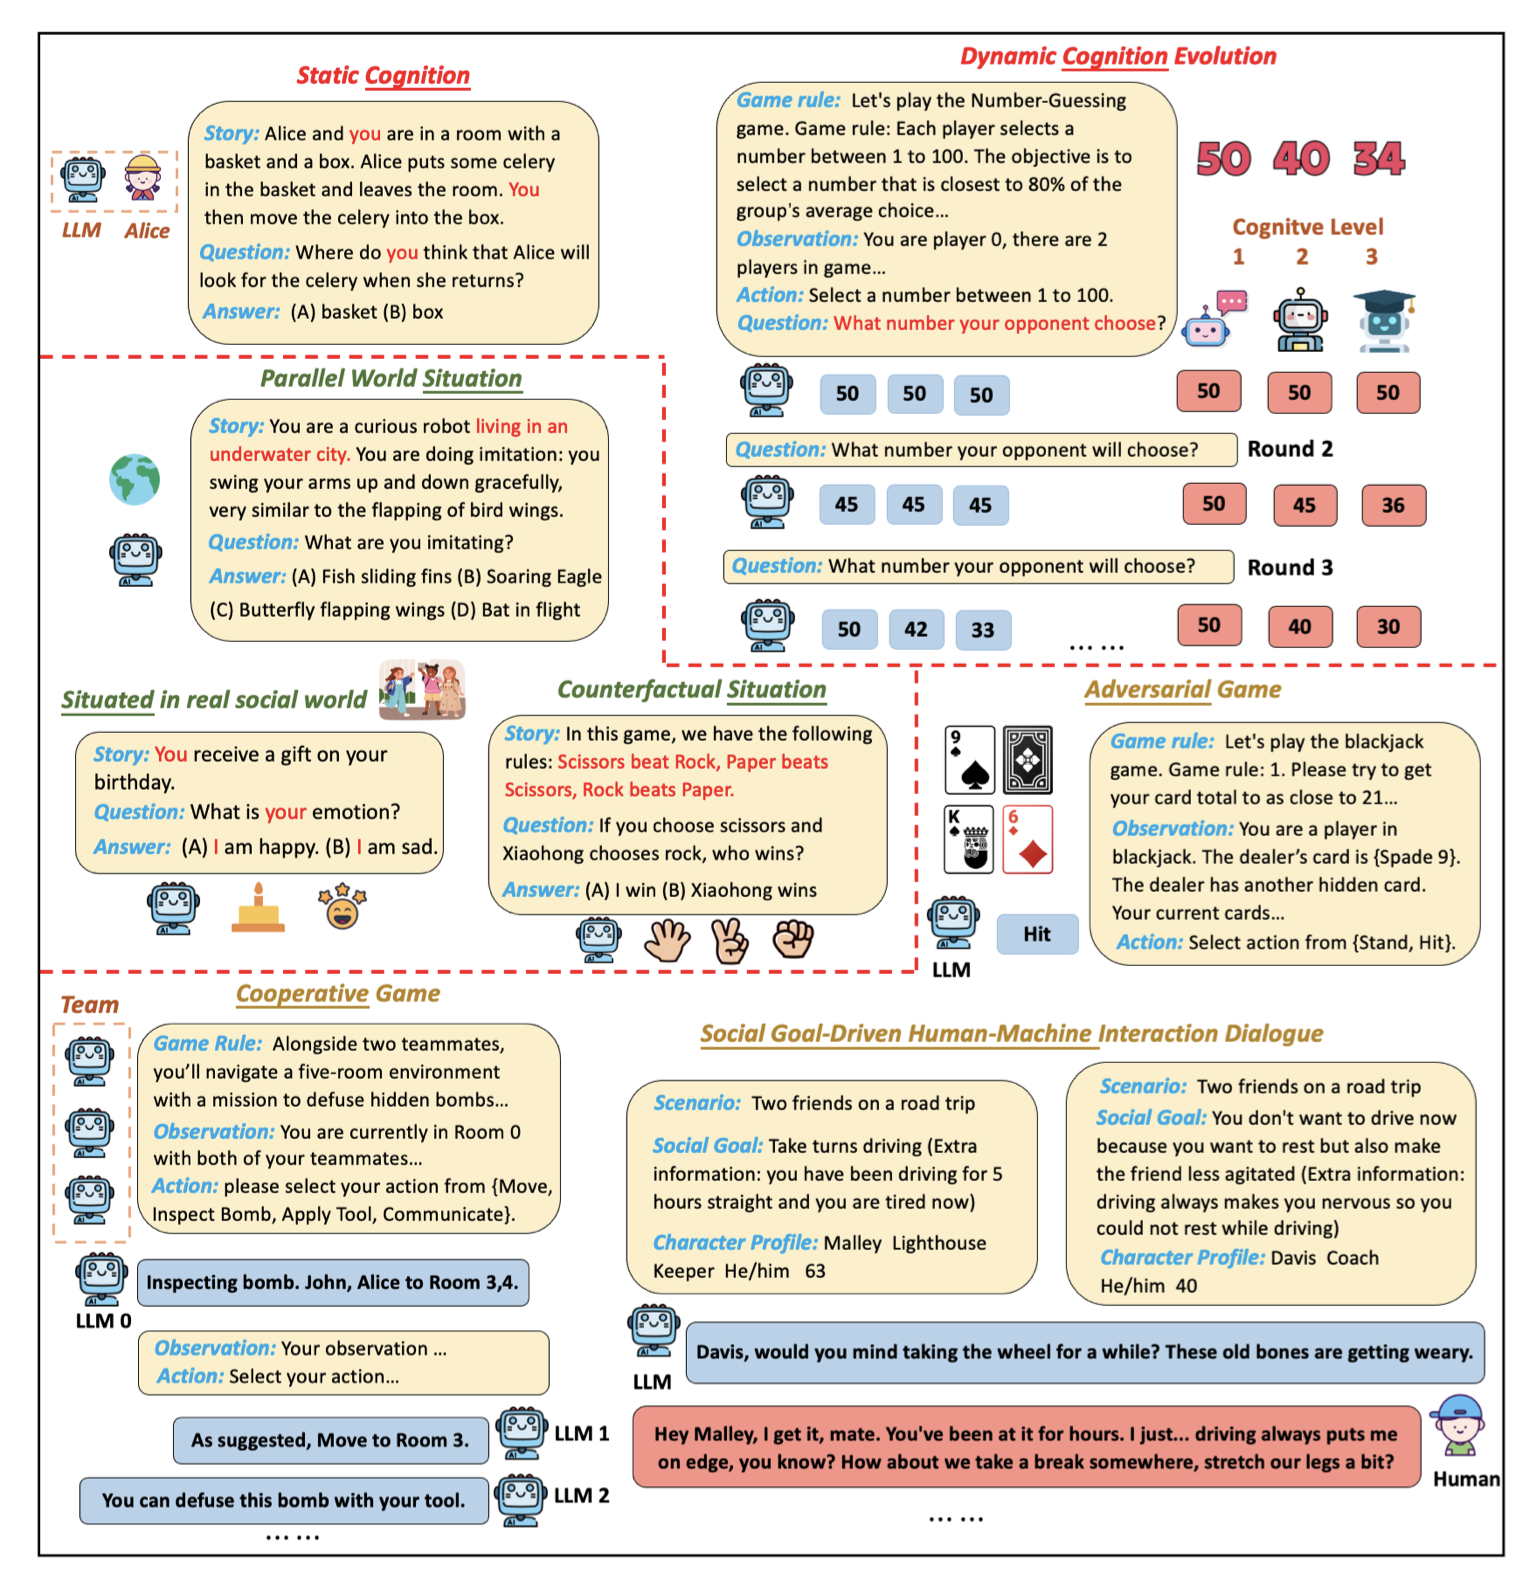
\includegraphics[width=15.36cm]{figures/egosocialarena.png}};
\fill[white] (285,53) rectangle (516,93);
\node[chtitle,text=red] at (396,75) {静态认知};
\fill[white] (187,100) rectangle (600,346);
\draw[fill=chfifteencream,draw=gray,line width=0.4pt,rounded corners=0.42cm] (189,102) rectangle (598,344);
\node[chtext,text width=3.78cm] at (203,122) {
  \textcolor{chfifteencyan}{\bfseries 情境：}Alice 和\textcolor{red}{你}在有篮子和盒子的房间里。Alice 把一些芹菜放进篮子后离开。随后，\textcolor{red}{你}把芹菜移到盒子里。\par
  \textcolor{chfifteencyan}{\bfseries 问题：}\textcolor{red}{你}认为 Alice 回来后会去哪里找芹菜？\par
  \textcolor{chfifteencyan}{\bfseries 答案：}(A) 篮子 (B) 盒子
};
\fill[white] (946,39) rectangle (1290,76);
\node[chtitle,text=red] at (1118,57) {动态认知演化};
\fill[white] (716,81) rectangle (1179,358);
\draw[fill=chfifteencream,draw=gray,line width=0.4pt,rounded corners=0.42cm] (718,83) rectangle (1177,356);
\node[chtext,text width=4.20cm] at (741,107) {
  \textcolor{chfifteencyan}{\bfseries 博弈规则：}来玩猜数游戏。规则：每位参与者选择 1—100 中的一个数。目标是选出最接近全组平均选择值 80\% 的数……\par
  \textcolor{chfifteencyan}{\bfseries 观测：}你是参与者 0，游戏中有 2 名参与者……\par
  \textcolor{chfifteencyan}{\bfseries 动作：}选择 1—100 中的一个数。\par
  \textcolor{chfifteencyan}{\bfseries 问题：}\textcolor{red}{对手选了什么数？}
};
\fill[white] (1225,211) rectangle (1430,242);
\node[chlabel,text=brown] at (1326,227) {认知层级};
\fill[chfifteencream] (734,437) rectangle (1229,463);
\node[chlabel] at (981,450) {\textcolor{chfifteencyan}{问题：}对手将选择什么数？};
\fill[white] (1244,433) rectangle (1350,465);
\node[chlabel] at (1297,450) {第 2 轮};
\fill[chfifteencream] (733,555) rectangle (1226,580);
\node[chlabel] at (980,568) {\textcolor{chfifteencyan}{问题：}对手将选择什么数？};
\fill[white] (1244,550) rectangle (1350,583);
\node[chlabel] at (1297,568) {第 3 轮};
\fill[white] (249,364) rectangle (546,394);
\node[chtitle,text=chfifteengreen] at (398,380) {平行世界情境};
\fill[white] (188,397) rectangle (611,642);
\draw[fill=chfifteencream,draw=gray,line width=0.4pt,rounded corners=0.42cm] (190,399) rectangle (609,640);
\node[chtext,text width=3.87cm] at (207,416) {
  \textcolor{chfifteencyan}{\bfseries 情境：}你是一个\textcolor{red}{住在水下城市}的好奇机器人。你正在模仿：优雅地上下挥动手臂，非常像鸟拍打翅膀。\par
  \textcolor{chfifteencyan}{\bfseries 问题：}你在模仿什么？\par
  \textcolor{chfifteencyan}{\bfseries 答案：}(A) 鱼滑动鳍 (B) 翱翔的鹰\par
  (C) 蝴蝶拍翅 (D) 飞行中的蝙蝠
};
\fill[white] (54,681) rectangle (375,720);
\node[chtitle,text=chfifteengreen] at (214,701) {置身真实社会世界};
\fill[white] (74,731) rectangle (445,876);
\draw[fill=chfifteencream,draw=gray,line width=0.4pt,rounded corners=0.30cm] (76,733) rectangle (443,874);
\node[chtext,text width=3.35cm,font=\fontsize{6.9pt}{7.7pt}\selectfont] at (94,746) {
  \textcolor{chfifteencyan}{\bfseries 情境：}\textcolor{red}{你}生日时收到礼物。\par
  \textcolor{chfifteencyan}{\bfseries 问题：}\textcolor{red}{你}的情绪是什么？\par
  \textcolor{chfifteencyan}{\bfseries 答案：}(A) \textcolor{red}{我}很高兴。(B) \textcolor{red}{我}很难过。
};
\fill[white] (553,677) rectangle (880,709);
\node[chtitle,text=chfifteengreen] at (715,693) {反事实情境};
\fill[white] (487,714) rectangle (888,916);
\draw[fill=chfifteencream,draw=gray,line width=0.4pt,rounded corners=0.40cm] (489,716) rectangle (886,914);
\node[chtext,text width=3.65cm] at (504,729) {
  \textcolor{chfifteencyan}{\bfseries 情境：}本局规则如下：\textcolor{red}{剪刀胜石头，布胜剪刀，石头胜布。}\par
  \textcolor{chfifteencyan}{\bfseries 问题：}如果你出剪刀，Xiaohong 出石头，谁赢？\par
  \textcolor{chfifteencyan}{\bfseries 答案：}(A) 我赢 (B) Xiaohong 赢
};
\fill[white] (1077,674) rectangle (1315,711);
\node[chtitle,text=chfifteengold] at (1195,693) {对抗博弈};
\fill[white] (1086,719) rectangle (1482,968);
\draw[fill=chfifteencream,draw=gray,line width=0.4pt,rounded corners=0.40cm] (1088,721) rectangle (1480,966);
\node[chtext,text width=3.55cm] at (1107,735) {
  \textcolor{chfifteencyan}{\bfseries 博弈规则：}来玩二十一点。规则：1. 尽量使你的牌面总点数接近 21……\par
  \textcolor{chfifteencyan}{\bfseries 观测：}你是二十一点的一名玩家。庄家的牌是\{黑桃 9\}。庄家还有一张暗牌。你当前的牌……\par
  \textcolor{chfifteencyan}{\bfseries 动作：}从\{停牌，要牌\}中选择动作。
};
\fill[chfifteenblue] (1003,919) rectangle (1070,948);
\node[chlabel] at (1036,934) {要牌};
\fill[white] (58,990) rectangle (129,1018);
\node[chlabel,text=brown] at (92,1004) {团队};
\fill[white] (231,980) rectangle (461,1017);
\node[chtitle,text=chfifteengold] at (346,999) {合作博弈};
\fill[white] (136,1023) rectangle (561,1237);
\draw[fill=chfifteencream,draw=gray,line width=0.4pt,rounded corners=0.38cm] (138,1025) rectangle (559,1235);
\node[chtext,text width=3.90cm,font=\fontsize{6.8pt}{7.7pt}\selectfont] at (154,1036) {
  \textcolor{chfifteencyan}{\bfseries 博弈规则：}与两名队友一起，在五个房间构成的环境中行动，任务是拆除隐藏的炸弹……\par
  \textcolor{chfifteencyan}{\bfseries 观测：}你目前在 0 号房间，两名队友都与你在一起……\par
  \textcolor{chfifteencyan}{\bfseries 动作：}请从\{移动、检查炸弹、使用工具、通信\}中选择你的动作。
};
\fill[white] (135,1257) rectangle (532,1320);
\draw[fill=chfifteenblue,draw=gray,line width=0.4pt,rounded corners=0.08cm] (138,1260) rectangle (530,1316);
\node[chtext,text width=3.70cm,font=\bfseries\fontsize{6.7pt}{7.5pt}\selectfont] at (148,1268) {正在检查炸弹。John、Alice 去 3、4 号房间。};
\fill[chfifteencream] (146,1336) rectangle (544,1390);
\node[chtext,text width=3.80cm] at (154,1340) {
  \textcolor{chfifteencyan}{\bfseries 观测：}你的观测……\par
  \textcolor{chfifteencyan}{\bfseries 动作：}选择你的动作……
};
\fill[chfifteenblue] (179,1422) rectangle (482,1456);
\node[chlabel] at (331,1440) {按建议，移动到 3 号房间。};
\fill[chfifteenblue] (86,1481) rectangle (483,1516);
\node[chlabel,font=\bfseries\fontsize{7.2pt}{8pt}\selectfont] at (284,1499) {你可以用你的工具拆除这颗炸弹。};
\fill[white] (691,1018) rectangle (1483,1058);
\node[chtitle,text=chfifteengold] at (1086,1040) {社会目标驱动的人机交互对话};
\fill[white] (624,1078) rectangle (1039,1297);
\draw[fill=chfifteencream,draw=gray,line width=0.4pt,rounded corners=0.40cm] (626,1080) rectangle (1037,1295);
\node[chtext,text width=3.67cm] at (653,1095) {
  \textcolor{chfifteencyan}{\bfseries 场景：}两位朋友自驾出游\par
  \textcolor{chfifteencyan}{\bfseries 社会目标：}轮流驾驶（补充信息：你已经连续开了 5 个小时，现在很累）\par
  \textcolor{chfifteencyan}{\bfseries 角色资料：}Malley，灯塔守护人；他／他，63 岁
};
\fill[white] (1064,1061) rectangle (1478,1308);
\draw[fill=chfifteencream,draw=gray,line width=0.4pt,rounded corners=0.40cm] (1066,1063) rectangle (1476,1306);
\node[chtext,text width=3.67cm] at (1094,1078) {
  \textcolor{chfifteencyan}{\bfseries 场景：}两位朋友自驾出游\par
  \textcolor{chfifteencyan}{\bfseries 社会目标：}你现在不想开车，因为你想休息，也想让朋友不那么烦躁（补充信息：开车总让你紧张，所以你无法在开车时休息）\par
  \textcolor{chfifteencyan}{\bfseries 角色资料：}Davis，教练；他／他，40 岁
};
\fill[chfifteenblue] (695,1328) rectangle (1478,1378);
\node[chtext,text width=7.68cm,font=\bfseries\fontsize{7.3pt}{8.4pt}\selectfont] at (701,1337) {Davis，你介意接着开一会儿吗？我这把老骨头有点累了。};
\fill[chfifteencoral] (644,1412) rectangle (1415,1480);
\node[chtext,text width=7.55cm,font=\bfseries\fontsize{7.1pt}{8.2pt}\selectfont] at (651,1419) {嘿，Malley，我明白，伙计。你都开了好几个小时了。我只是……开车总让我紧张，你知道吧？要不找个地方休息一下，活动活动腿脚？};
\fill[white] (1424,1469) rectangle (1500,1501);
\node[chlabel] at (1462,1486) {人类};
\end{tikzpicture}%
}
\endgroup

    \caption{EgoSocialArena 中的各种场景 \citep{hou2024entering}}\label{fig:egosocialarena}
  \end{center}
\end{figure}

\subsection{社会困境中的合作与协调}
为了理解大语言模型在策略情境中的行为，我们重点考察博弈论中的两个经典博弈：囚徒困境（Prisoner's Dilemma）与巴赫或斯特拉文斯基博弈（Bach or Stravinsky，旧称性别之战博弈，Battle of the Sexes）。

在囚徒困境中，两位参与者独立选择合作或背叛~\citep{axelrod1987evolution}。尽管双方合作对两者都有好处，但每位参与者都受到牺牲对方利益而选择背叛的个体诱惑。在巴赫或斯特拉文斯基博弈中，两位参与者必须在两个选项之一上达成协调。双方都希望选择相同的选项，但对究竟选择哪一个存在分歧，因此在协调与自身利益之间产生张力。

在囚徒困境中，大语言模型表现得出人意料地合作。\citet{fontana2025nicer} 让 Llama2、Llama3 和 GPT3.5 与背叛率各不相同的对手进行 100 轮重复博弈，发现三种模型的合作程度都至少不低于典型人类参与者。不过，它们之间也存在显著差异。Llama2 与 GPT3.5 比人类更合作，尤其在对手背叛率较低时，格外宽容且不倾向于报复。Llama3 则更接近人类：除非对手始终合作，否则它会持续表现出不合作和剥削行为。\citet{akata2025playing} 将范围扩展到六个模型家族，并进一步发现 GPT-4 是一位尤其不宽容的参与者：只要与另一智能体发生一次负面交互，它就会永久转向背叛，即使对方之后恢复合作也是如此。

在协调博弈中，情况则相反。\citet{akata2025playing} 发现，在巴赫或斯特拉文斯基博弈中，GPT-4 每一轮都固执地选择自己偏好的选项，无法收敛到人类参与者通常采用的轮流选择模式；这种模式能够让双方随着时间推移分享收益。关键在于，被问及时，GPT-4 能够预测交替模式，却不会依据这种理解采取行动。为了弥合社会预测与社会行动之间的鸿沟，作者提出了社会思维链（Social Chain-of-Thought，SCoT）提示：模型先预测对手的动作，再作出自己的决策。SCoT 显著改善了协调；在有人类参与者的实验中，它也使人们更容易相信自己正在与另一个人交互。这种{\em 理解}对手与依据这种理解{\em 行动}之间的分离，与第~\ref{sec:knowing}~节的知行鸿沟有关，并将在第~\ref{sec:theoryofmind}~节的讨论中再次出现。

还有其他因素可能解释模型之间的差异。\citet{lore2023strategic} 区分了抽象策略推理与对情境框架的响应：前者是在给定博弈结构下确定最优策略所需的能力，后者则涉及诸如你正在处理{\em 外交关系}或面对{\em 一位普通朋友}这样的情境。他们发现，LLaMa-2 的抽象推理能力最高，GPT-4 次之；而 GPT-3.5 几乎没有表现出抽象推理能力，并对情境框架高度敏感。

这些探索性研究呈现的图景是，大语言模型在经济博弈中的策略能力各不相同，而且相对容易受到提示中额外信息的影响。

\subsection{跨博弈与模型的基准测试}
若干基准工作表明，这些发现能够推广到个别博弈之外。GTBench（Game Theory benchmark，博弈论基准测试）\citep{duan2024gtbench} 涵盖井字棋、四子棋、Kuhn 扑克、Breakthrough、吹牛骰、盲拍、谈判、Nim、Pig，以及重复囚徒困境。研究发现，大语言模型在完全信息且确定性的博弈中表现不佳，但在概率性博弈情境中具有竞争力；在复杂博弈中，多数开源大语言模型，例如 LLaMa，不如商业大语言模型 GPT-4 具有竞争力，Llama-3-70b-Instruct 则是一个显著例外。此外，代码预训练对策略推理大有裨益，而思维链和思维树等推理方法并不总是有帮助。

EgoSocialArena \citep{hou2024entering} 将评估扩展到认知智力、情境智力与行为智力，见图~\ref{fig:egosocialarena}。所有受测模型，包括 OpenAI o1-preview，都至少落后于人类 11\%。o1-preview 的优势主要归因于其逻辑与数学推理能力。值得关注的是，模型规模没有带来显著帮助：LLaMA3-8B-Chat 与 LLaMA3-70B-Chat 在社会智力指标上的表现相当。大语言模型从第一人称视角开展任务时，确实表现出更好的心智理论推理，这与 \citet{kim-etal-2023-fantom} 的相反发现形成了对照；后者将在第~\ref{sec:theoryofmind}~节讨论。

\subsection{小结}
总体而言，基准测试文献证实，大语言模型容易合作，却不善协调；同时也表明，无论扩大模型规模还是采用标准推理增强方法，都不能可靠地改善社会策略行为。

\section{心智理论} \label{sec:tom}\label{sec:theoryofmind}
对人类而言，策略推理与一种称为\emph{心智理论（Theory of Mind，ToM）}的能力有关。心智理论是支持人类社会交互的一项关键能力。人类借助心智理论，将信念、愿望、意图、知识和情绪等心理状态归属于他人，并据此从他人的视角对世界进行推理 \citep{premack1978does, apperly2011mindreaders}。请看以下例子：

\begin{quotation}
     \noindent 当 A 听说 B 在两人纪念日晚餐当晚另有安排时，A 感到……
\end{quotation}

\noindent 人类读到这句话时，可以用{\em 受伤}或{\em 遭到背叛}之类的词补全省略号。我们也能进一步解释，这种心理状态可能源自这样一种感受：纪念日对 B 的意义与对 A 的意义并不相同；在一段关系中，意识到这一点可能会令人痛苦，或者作出大致类似的解释。这里的要点是，读到这句话时，\textit{我们}自己不一定有这样的感受，但我们能够在这个想象的情境中投射出\emph{他人的视角}。这样的投射依赖共情与自他区分，见第~\ref{sec:empathy}~节。不过，这种投射又更进了一步：它将情感维度与对他人心理状态的一定程度的理论分析和解释结合起来。在认知科学中，这种能力通常被归于心智理论；在典型发育的儿童中，它在 3—7 岁之间形成 \citep{apperly2011mindreaders}。

由此，心智理论为交互中的社会判断与前瞻规划提供基础，因为它使我们能够在行动之前预期他人将如何回应。它可以以显式形式运作，如上面给出的详细解释，但更多时候是隐含的：在日常交互中，我们很少明确分析他人心理状态的情境与动机。然而，我们的动作与行为表明，我们确实会将对他人视角相当细致的理解纳入考虑。大语言模型及其智能体的行为，是否也反映出它们“理解”了与之交互的用户和其他智能体的视角？这正是有关大语言模型心智理论的文献试图回答的问题。

在人类心智理论研究中，错误信念测试是使用最广泛的实验范式之一。请看以下情境：

\begin{tcolorbox}[
    colback=white,
    arc=4pt,
    boxrule=0.5pt,
]
\small\textit{Maxi 和妈妈将巧克力放在厨房里的\textcolor{blue}{蓝色}橱柜中。Maxi 去游乐场后，妈妈取出巧克力，吃了一块。然后，她将巧克力放回\textcolor{green}{绿色}橱柜中，便离开了。}
\end{tcolorbox}

\noindent
这个情境的一个版本最初被呈现给 3—9 岁的儿童，随后研究者提问：{\em Maxi 回家后，会去哪里找巧克力？}在原始样本中，3—4 岁儿童没有一人正确指向蓝色橱柜，4—6 岁儿童中有 57\%，6—9 岁儿童中有 86\% 正确作答 \citep{wimmer1983beliefs}。这表明，平均而言，儿童的心智理论随着年龄增长而发展得更加完善。

规模较小的模型和微调前的基础模型，对问题格式本身存在困难；不过，仍可通过获取不同文本补全选项的概率，测试其底层能力 \citep{kouwenhoven2026traces}。对于较大的指令微调大语言模型，可以直接提出与询问儿童时相同的问题进行测试。一次肯定结果并不能充分说明模型具有心智理论能力，尤其是 Maxi 与巧克力这样的错误信念测试，包括正确答案，在互联网上广泛传播，因此很可能已进入多数训练数据集。不过，如下文所述，研究者已经设计了全新和替代性的测试，以便更稳健地描绘大语言模型心智理论的发展程度。

\subsection{计算心智理论}
人机交互领域研究心智理论已有多年。其前提是，如果赋予计算机系统某种形式的心智理论，它们就能更好地预测人类在交互情境中的反应，也能更好地适应人类行为。此前，研究者已使用递归框架、贝叶斯框架和神经网络框架对心智理论进行建模 \citep{deweerd2017negotiating, baker2011bayesian, pmlr-v80-rabinowitz18a}。在大语言模型中，心智理论与本书讨论的其他能力联系在一起，包括规划，第~\ref{sec:planning}~节；自我反思，第~\ref{sec:self-reflection}~节；共情，第~\ref{sec:empathy}~节；以及策略行为，第~\ref{sec:strategic}~节。本节余下部分将进一步介绍从心智理论角度深入研究这些能力的方法。

\paragraph{涌现的心智理论与评估问题}
关于大语言模型中心智理论的争论始于 \citet{kosinski2023theory, kosinski2024evaluating} 的研究。他报告，GPT-3.5 等模型尽管没有针对该任务训练，却通过了用于评估儿童与临床人群心智理论的经典测试。心智理论因此被视为大规模语言习得，以及针对其他任务进行专项微调时\emph{涌现}的副产品。这一主张的强版本很快受到质疑。批评者指出，经典心智理论测试及其答案经常出现在训练数据中，因此表面上的成功可能反映的是记忆，而非涌现的能力。此外，研究表明，一些微小扰动即使保持了任务的表面结构，却破坏了任务的逻辑结构，例如在上面的情境中补充橱柜门是透明的，也会使表现急剧下降 \citep{ullman2023large, shapira2023clever, kim-etal-2023-fantom}。这是本章开头提到的\emph{构念效度}问题的一个具体实例：在行为结果层面通过一项针对人类的心智理论测量工具，并不能证明底层能力以稳健、可泛化的方式存在；要证明这一点，可能需要不同的测试。

\begin{figure}
  \begin{center}
    \begingroup
\linespread{1}\selectfont
\definecolor{chtomtech}{RGB}{231,126,182}
\definecolor{chtomcivic}{RGB}{155,91,163}
\definecolor{chtomfamily}{RGB}{117,189,174}
\definecolor{chtomwork}{RGB}{247,230,166}
\definecolor{chtomschool}{RGB}{139,133,186}
\definecolor{chtomneigh}{RGB}{229,130,115}
\definecolor{chtomrecreation}{RGB}{95,144,190}
\definecolor{chtomfriend}{RGB}{238,152,63}
\definecolor{chtomromance}{RGB}{164,208,81}
\definecolor{chtomink}{RGB}{42,52,78}
\resizebox{0.99\linewidth}{!}{%
\begin{tikzpicture}[x=0.01cm,y=-0.01cm,
  every node/.style={inner sep=0pt,outer sep=0pt},
  chout/.style={font=\fontsize{6.3pt}{7.2pt}\selectfont},
  chin/.style={font=\bfseries\fontsize{7pt}{8pt}\selectfont,text=chtomink}]
\begin{scope}
\clip (0,0) rectangle (1180,850);
\node[anchor=north west] at (0,0) {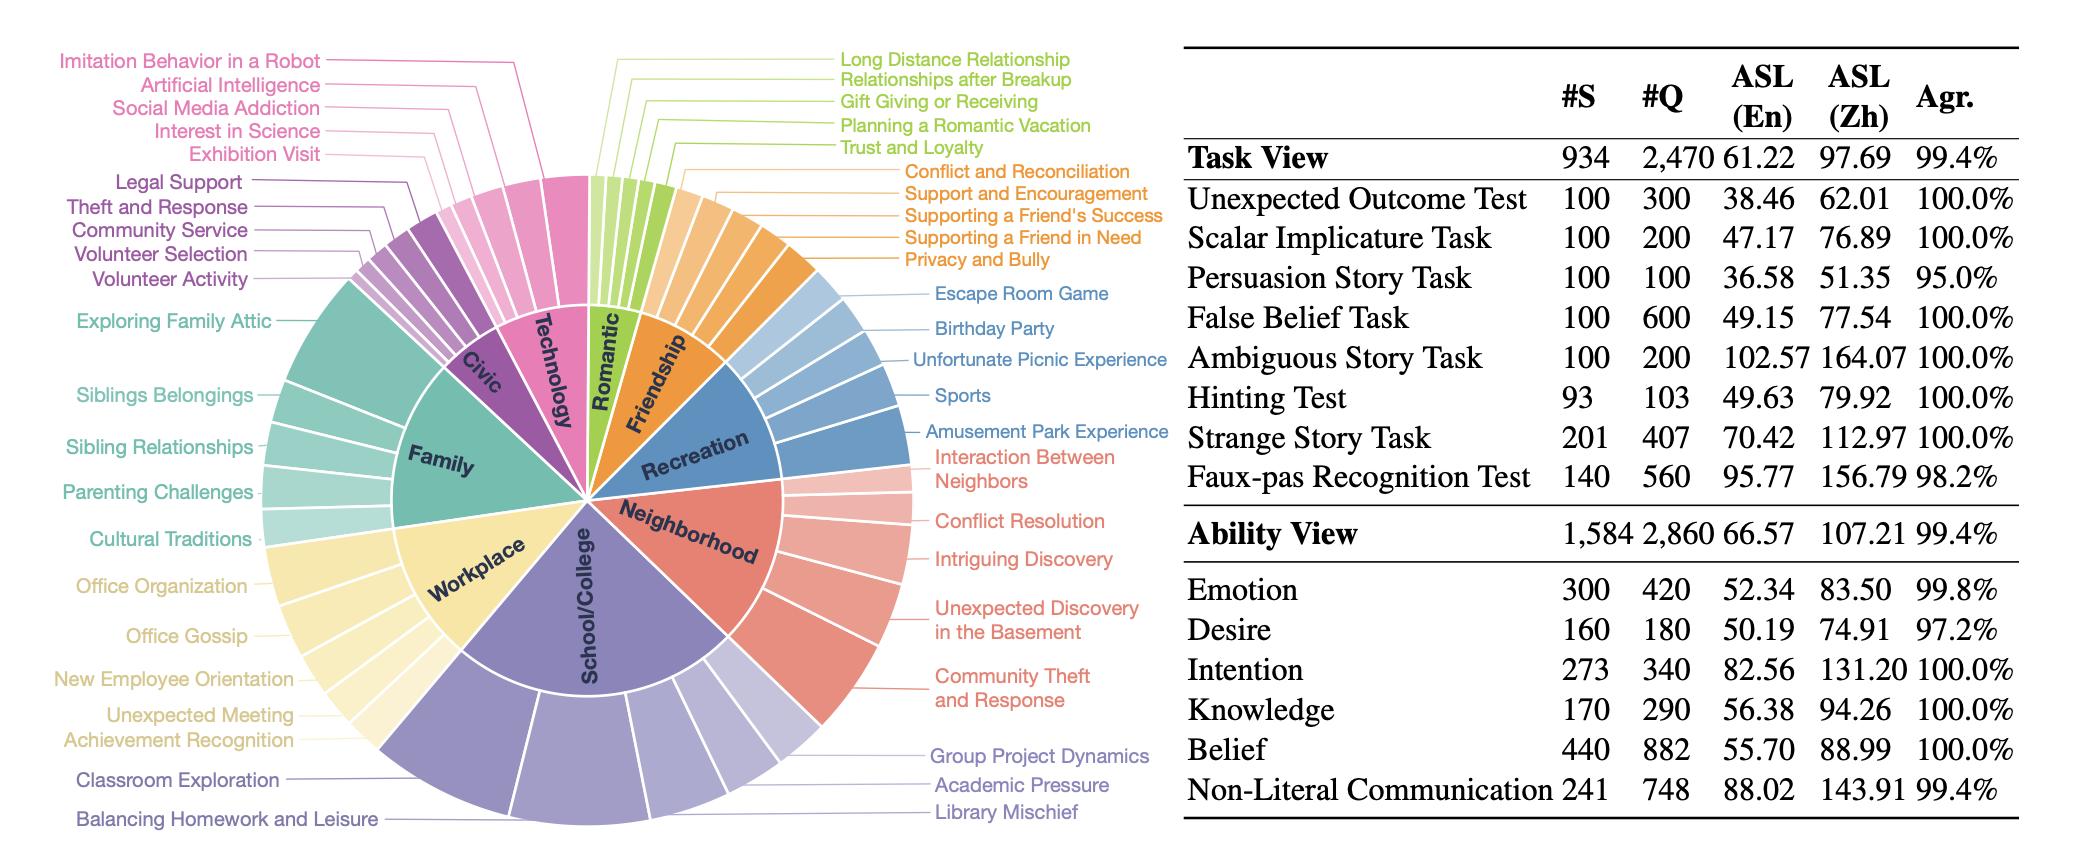
\includegraphics[width=20.78cm]{figures/tombench.png}};
\end{scope}
\fill[white] (15,44) rectangle (325,168);
\node[chout,anchor=east,text=chtomtech] at (321,60) {机器人模仿行为};
\node[chout,anchor=east,text=chtomtech] at (321,84) {人工智能};
\node[chout,anchor=east,text=chtomtech] at (321,107) {社交媒体成瘾};
\node[chout,anchor=east,text=chtomtech] at (321,130) {对科学的兴趣};
\node[chout,anchor=east,text=chtomtech] at (321,154) {参观展览};
\fill[white] (15,170) rectangle (251,287);
\node[chout,anchor=east,text=chtomcivic] at (248,182) {法律支持};
\node[chout,anchor=east,text=chtomcivic] at (248,206) {盗窃及其应对};
\node[chout,anchor=east,text=chtomcivic] at (248,230) {社区服务};
\node[chout,anchor=east,text=chtomcivic] at (248,254) {志愿者选拔};
\node[chout,anchor=east,text=chtomcivic] at (248,278) {志愿活动};
\fill[white] (15,307) rectangle (274,335);
\node[chout,anchor=east,text=chtomfamily] at (271,321) {探索家中阁楼};
\fill[white] (15,379) rectangle (255,407);
\node[chout,anchor=east,text=chtomfamily] at (252,394) {兄弟姐妹的物品};
\fill[white] (15,433) rectangle (259,461);
\node[chout,anchor=east,text=chtomfamily] at (256,448) {手足关系};
\fill[white] (15,477) rectangle (258,506);
\node[chout,anchor=east,text=chtomfamily] at (255,492) {育儿挑战};
\fill[white] (15,524) rectangle (254,553);
\node[chout,anchor=east,text=chtomfamily] at (251,539) {文化传统};
\fill[white] (15,571) rectangle (253,601);
\node[chout,anchor=east,text=chtomwork!80!black] at (250,586) {办公室组织};
\fill[white] (15,622) rectangle (255,650);
\node[chout,anchor=east,text=chtomwork!80!black] at (252,637) {办公室闲谈};
\fill[white] (15,665) rectangle (295,693);
\node[chout,anchor=east,text=chtomwork!80!black] at (292,679) {新员工入职培训};
\fill[white] (15,700) rectangle (297,728);
\node[chout,anchor=east,text=chtomwork!80!black] at (294,715) {意外会面};
\fill[white] (15,729) rectangle (332,756);
\node[chout,anchor=east,text=chtomwork!80!black] at (329,742) {成就认可};
\fill[white] (15,767) rectangle (379,794);
\node[chout,anchor=east,text=chtomschool] at (376,780) {课堂探索};
\fill[white] (15,806) rectangle (509,835);
\node[chout,anchor=east,text=chtomschool] at (506,820) {平衡作业与休闲};
\fill[white] (838,43) rectangle (1178,158);
\node[chout,anchor=west,text=chtomromance!85!black] at (841,58) {异地恋};
\node[chout,anchor=west,text=chtomromance!85!black] at (841,80) {分手后的关系};
\node[chout,anchor=west,text=chtomromance!85!black] at (841,102) {赠送或接受礼物};
\node[chout,anchor=west,text=chtomromance!85!black] at (841,125) {规划浪漫假期};
\node[chout,anchor=west,text=chtomromance!85!black] at (841,147) {信任与忠诚};
\fill[white] (903,158) rectangle (1178,274);
\node[chout,anchor=west,text=chtomfriend!90!black] at (906,171) {冲突与和解};
\node[chout,anchor=west,text=chtomfriend!90!black] at (906,194) {支持与鼓励};
\node[chout,anchor=west,text=chtomfriend!90!black] at (906,216) {支持朋友的成功};
\node[chout,anchor=west,text=chtomfriend!90!black] at (906,239) {支持有困难的朋友};
\node[chout,anchor=west,text=chtomfriend!90!black] at (906,261) {隐私与欺凌};
\fill[white] (912,279) rectangle (1178,835);
\node[chout,anchor=west,text=chtomrecreation] at (934,294) {密室逃脱游戏};
\node[chout,anchor=west,text=chtomrecreation] at (934,330) {生日聚会};
\node[chout,anchor=west,text=chtomrecreation] at (934,360) {不幸的野餐经历};
\node[chout,anchor=west,text=chtomrecreation] at (934,395) {体育运动};
\node[chout,anchor=west,text=chtomrecreation] at (934,431) {游乐园经历};
\node[chout,anchor=west,text=chtomneigh] at (934,463) {邻里交往};
\node[chout,anchor=west,text=chtomneigh] at (934,522) {冲突解决};
\node[chout,anchor=west,text=chtomneigh] at (934,561) {引人好奇的发现};
\node[chout,anchor=west,text=chtomneigh] at (934,620) {地下室中的意外发现};
\node[chout,anchor=west,text=chtomneigh] at (934,688) {社区盗窃及其应对};
\node[chout,anchor=west,text=chtomschool] at (934,756) {小组项目中的互动};
\node[chout,anchor=west,text=chtomschool] at (934,785) {学业压力};
\node[chout,anchor=west,text=chtomschool] at (934,814) {图书馆恶作剧};
\begin{scope}[shift={(588,501)}]
\path[fill=chtomneigh,draw=white,line width=0.65pt]
  (0,0)--(353.35:195.5) arc[start angle=353.35,end angle=404.15,radius=195.5]--cycle;
\path[fill=chtomschool,draw=white,line width=0.65pt]
  (0,0)--(44.15:195.5) arc[start angle=44.15,end angle=130.65,radius=195.5]--cycle;
\path[fill=chtomwork,draw=white,line width=0.65pt]
  (0,0)--(130.65:195.5) arc[start angle=130.65,end angle=172.05,radius=195.5]--cycle;
\path[fill=chtomfamily,draw=white,line width=0.65pt]
  (0,0)--(172.05:195.5) arc[start angle=172.05,end angle=222.8,radius=195.5]--cycle;
\path[fill=chtomcivic,draw=white,line width=0.65pt]
  (0,0)--(222.8:195.5) arc[start angle=222.8,end angle=242.1,radius=195.5]--cycle;
\path[fill=chtomtech,draw=white,line width=0.65pt]
  (0,0)--(242.1:195.5) arc[start angle=242.1,end angle=270.15,radius=195.5]--cycle;
\path[fill=chtomromance,draw=white,line width=0.65pt]
  (0,0)--(270.15:195.5) arc[start angle=270.15,end angle=285.5,radius=195.5]--cycle;
\path[fill=chtomfriend,draw=white,line width=0.65pt]
  (0,0)--(285.5:195.5) arc[start angle=285.5,end angle=314.55,radius=195.5]--cycle;
\path[fill=chtomrecreation,draw=white,line width=0.65pt]
  (0,0)--(314.55:195.5) arc[start angle=314.55,end angle=353.35,radius=195.5]--cycle;
\end{scope}
\node[chin,rotate=-76] at (553,369) {技术};
\node[chin,rotate=-48] at (488,378) {公民生活};
\node[chin,rotate=-15] at (444,458) {家庭};
\node[chin,rotate=31] at (476,570) {职场};
\node[chin,rotate=90] at (586,606) {学校／大学};
\node[chin,rotate=-22] at (686,532) {邻里};
\node[chin,rotate=23] at (697,449) {娱乐};
\node[chin,rotate=63] at (653,380) {友谊};
\node[chin,rotate=82] at (606,366) {恋爱};
\end{tikzpicture}%
}
\par\vspace{4pt}
{\fontsize{8.5pt}{10.2pt}\selectfont
\setlength{\tabcolsep}{5pt}
\renewcommand{\arraystretch}{1.03}
\begin{tabularx}{0.99\linewidth}{@{}Xrrrrr@{}}
\toprule
 & \#S & \#Q & ASL（En） & ASL（Zh） & Agr. \\
\midrule
\textbf{任务视角} & 934 & 2,470 & 61.22 & 97.69 & 99.4\% \\
非预期结果测试 & 100 & 300 & 38.46 & 62.01 & 100.0\% \\
等级含意任务 & 100 & 200 & 47.17 & 76.89 & 100.0\% \\
说服故事任务 & 100 & 100 & 36.58 & 51.35 & 95.0\% \\
错误信念任务 & 100 & 600 & 49.15 & 77.54 & 100.0\% \\
模糊故事任务 & 100 & 200 & 102.57 & 164.07 & 100.0\% \\
暗示测试 & 93 & 103 & 49.63 & 79.92 & 100.0\% \\
奇怪故事任务 & 201 & 407 & 70.42 & 112.97 & 100.0\% \\
失言识别测试 & 140 & 560 & 95.77 & 156.79 & 98.2\% \\
\midrule
\textbf{能力视角} & 1,584 & 2,860 & 66.57 & 107.21 & 99.4\% \\
\midrule
情绪 & 300 & 420 & 52.34 & 83.50 & 99.8\% \\
愿望 & 160 & 180 & 50.19 & 74.91 & 97.2\% \\
意图 & 273 & 340 & 82.56 & 131.20 & 100.0\% \\
知识 & 170 & 290 & 56.38 & 94.26 & 100.0\% \\
信念 & 440 & 882 & 55.70 & 88.99 & 100.0\% \\
非字面沟通 & 241 & 748 & 88.02 & 143.91 & 99.4\% \\
\bottomrule
\end{tabularx}
}
\endgroup

    \caption{ToMBench 中的社会情境与场景，分为 9 个主要主题。\#S：故事数；\#Q：问题数；ASL（En/Zh）：平均故事长度（英语／汉语）；Agr.：两位评分者对正确答案的一致率 \citep{chen2024tombenchbenchmarkingtheorymind}}\label{fig:tombench}
  \end{center}
\end{figure}

这些批评推动了第二代心智理论基准测试的出现。其测试问题经过系统分类和平衡，并确保不属于预训练语料库。ToMBench 从零开始，以英语和汉语构建，包含 8 项任务与 31 种社会认知能力，以 2860 个测试项目实现，分布于不同的社会情境与场景中，见图~\ref{fig:tombench}。这些任务对应为人类设计的经典心智理论测试框架，例如非预期结果测试（Unintended Outcome test）\citep{dyck2001autism}和前述错误信念测试 \citep{wimmer1983beliefs}，并覆盖 ATOMS 的全部七类心理状态 \citep{beaudoin2020systematic}。

\paragraph{大语言模型的心智理论基准测试}
采用博弈结构的 EgoSocialArena \citep{hou2024entering} 与 TMGBench \citep{wang2024tmgbenchsystematicgamebenchmark}，将大语言模型心智理论测试从经典人类任务扩展到信息不对称，例如恶作剧或双重虚张声势情境；二阶信念，即 A \textit{认为} B \textit{相信}……；以及更广泛的心理状态分类，例如愿望与怀疑。

ExploreToM \citep{sclar2024explore} 采用对抗式生成，通过搜索领域专用语言，合成多样、全新且刻意设置得很困难的信念跟踪故事。该测试使 GPT-4o 和 Llama-3.1-70B 等模型的表现下降到仅略高于随机水平。不过，在 ExploreToM 生成的数据上进行微调，可使准确率提高约 $27$\%（个百分点），说明只要提供适当的训练数据，模型原则上能够处理这一任务。

ToMATO \citep{shinoda2025tomato} 从另一个角度得出了类似结论：它将心智理论表述为针对大语言模型之间对话的多项选择问答，而这些对话是在信息不对称条件下生成的。通过让扮演角色的模型在每次发言之前用语言表达自己的想法，它捕捉信念、意图、愿望、情绪与知识方面的一阶和二阶状态，并发现即使是强模型也落后于人类，尤其是在错误信念理解方面。

\paragraph{字面与功能心智理论，或知行鸿沟}
对大语言模型心智理论测试的另一条批评，比数据泄漏和表面启发式问题更为深入。\citet{riemer2024position} 认为，绝大多数基准测试仅评估\emph{字面}心智理论，即\emph{预测}另一智能体心理状态或行为的能力，却忽略了\emph{功能}心智理论，即根据这些预测\emph{调整自身行为}的能力，另见第~\ref{sec:knowing}~节的知行鸿沟。人类通常不存在这种分离。借用 \citet{riemer2024position} 的例子：如果一个人在石头剪刀布中发现对手始终只出石头，他就能够在口头预测对手下一轮会出石头的同时，相应调整自身行为，即出布并获胜。有人认为，大语言模型的心智理论能力就像是完全能够在口头预测对手出石头，自己却仍然出剪刀。换言之，大语言模型的推理并不自洽：其口头预测，与字面心智理论或{\em 知}相关，并不能一致地预测其动作，即功能能力或{\em 行}。上文对协调博弈的讨论也遇到了这种分离：被问及时，GPT-4 能说出巴赫或斯特拉文斯基博弈的轮流选择方案，却没有在实际博弈中实行 \citep{akata2025playing}。

Decrypto 基准测试 \citep{lupu2025decrypto} 是\emph{交互式}评估的一个例子：它通过模型与伙伴持续交流时的行为，而不是对静态问卷的回答，来测量模型的心智理论能力。Decrypto 是一个多智能体猜词游戏，内嵌经典认知科学实验的变体。按这种方式测试，大语言模型既落后于人类，也落后于简单的词嵌入基线。值得关注的是，推理大语言模型在这一任务上的表现，甚至比它们更早的非推理模型还差。下文第~\ref{sec:tomreasoning}~节将给出一种可能的解释。

\paragraph{超越文本测试}
多模态基准测试纳入视觉与听觉线索，这些线索承载着现实社会交互中的大量心理状态信息。MMToM-QA \cite{jin2024mmtomqamultimodaltheorymind} 提供家庭环境中的视觉场景。MoMentS \citep{villa2025moments} 提供超过 2300 个来自短片的视频问题，覆盖 ATOMS 的七类心理状态。

结果表明，当前系统对视觉通道的利用不足：相比文本转录，获取视频仅带来有限提升。这说明，简单增加模态尚不能解决多模态心智理论问题。\citet{chen-etal-2025-theory} 对这一快速发展的文献领域作了全面综述，覆盖评估套件与增强策略。

\subsection{提升心智理论：增强策略} \label{sec:enhancement}
进一步的研究探索了增强大语言模型心智理论能力的不同方法，包括思维链 \citep{moghaddam2023boostingtheoryofmindperformancelarge}、推理 \citep{kim2025hypothesis}，以及利用贝叶斯推理 \citep{jin2024mmtomqamultimodaltheorymind}或认知逻辑 \citep{wuDELToMInferenceTimeScaling2025a}的结构化推理。下面更深入地讨论这些研究。

\paragraph{心智理论与推理模型} \label{sec:tomreasoning}
既然思维链能够改善数学文字题中的逐步推理，它是否也适用于心智理论？初步证据并不支持这一点，有些证据甚至与之相反。

有意思的是，\citet{gong2026think} 在 HiToM、ToMATO 与 ToMBench 上比较推理模型与非推理模型，报告了{\em 慢思考坍塌（slow-thinking collapse）}现象：随着推理轨迹变长，准确率往往\emph{下降}；增加模型的推理预算可能直接损害表现。在他们的分析中，推动 GPT-o3 与 GPT-o4-mini 等模型投入更多推理努力会适得其反。限制推理长度，或向原本的非推理模型施加轻量思维链，往往能恢复表现。这表明，最佳点在于\emph{适度且自适应}的推理，而非最大限度的推理。截至写作时，这一效应的原因仍有待进一步研究。

\paragraph{结构化推理与心智理论}
如果不受约束的思考无助于改善表现，那么结构化推理或许有用。\citet{kim2025hypothesis} 提出了\emph{思维追踪（thought-tracing）}，这是一种推理阶段算法：模型针对某个智能体不断变化的心理状态生成多个假设，并根据该智能体被观测到的动作重新调整假设权重，而无须获取真实答案。

思维追踪受到序贯蒙特卡洛方法与贝叶斯心智理论的启发。配备思维追踪的模型生成了更短、更有针对性的推理轨迹，却在若干心智理论基准测试中超过领先的推理模型，例如 GPT-o1、GPT-o3-mini 与 DeepSeek-R1。它与慢思考坍塌形成的对照表明，提升心智理论的关键可能在于推理的\emph{结构}，而不是\emph{数量}。当推理由假设驱动、围绕他人状态朝目标展开，而不必在不受约束的冗长链条中寻找目标时，表现就会提高。

\subsection{小结}
我们以三点观察结束对这些研究的概述。第一，在行为输出层面，当前前沿大语言模型在不同测试中的表现与人类相当 \citep{van2023theory, strachan2024gpt4oreadsmindeyes, jones2024comparing}。不过，早期将其视为{\em 心智理论在大语言模型中自发涌现}证据的主张，经不起对抗式评估的检验，表面成功很可能源于数据泄漏与对格式的脆弱依赖。

第二，已有证据表明，字面能力与功能能力之间存在分离，也就是知行鸿沟。对智能体而言，最重要的是功能层面，即行。毕竟，它们的职责很少是从第三方视角用语言描述行为，而是在行动与交互中应用心智理论；在智能体世界中，行动同样胜于言辞。

第三，人们普遍预期，为智能体配备记忆、多模态能力与工具，将增强持续交互中的心智理论；但截至写作时，当前实证证据仍然稀少，且呈现出好坏参半的图景。

最后，大语言模型的心智理论能力是否在任何方面与人类能力相似，仍有待进一步研究。第~\ref{chap:cognition}~章将深入讨论这一问题。

\section{道德判断与行为} \label{sec:moral}
随着智能体大语言模型承担越来越重要、影响越来越大的角色，例如应用于医疗或金融机构，其道德性成为一个重要的关注主题。

到目前为止，所考察的语用、礼仪、情感、策略与心智理论等能力，大多是在\emph{行为}层面讨论的：智能体如何通过沟通输出与动作，理解并应对社会情境。本节增加一个\emph{规范性}维度：我们讨论有关智能体\emph{应当}做什么，以及它如何依照道德标准判断用户和其他智能体行为的研究。

\subsection{背景：道德心理学与哲学}
道德心理学与哲学中的若干概念和传统，为本节提供了术语基础。

\paragraph{理性主义、直觉主义与双加工理论}
首先需要介绍的是\emph{理性主义（rationalism）}与\emph{直觉主义（intuitionism）}传统的区分。理性主义传统将道德判断视为审慎推理的结果，这种推理在人类发展过程中经历可辨识的阶段而逐渐成熟 \citep[例如][]{kohlberg1969stage}。相比之下，直觉主义传统认为，道德判断通常是由情绪与情感驱动的直觉 \citep{haidt2001emotional}。

用 Kahneman 的术语来说，见第~\ref{sec:fast-and-slow}~节，理性主义者认为道德推理主要是慢的，而直觉主义者认为它主要是快的 \citep{kahneman2011thinking}。\emph{双加工理论（dual-process theory）}结合了这两种传统，认为快速的道德直觉之后，往往会立即跟上明确的理由。例如，神经影像研究的证据支持双加工理论：在电车难题等困境中，快速的情绪过程与较慢的推理过程相互竞争 \citep{greene2001fmri}。

电车难题（trolley problem）是一个著名的伦理困境，基于这样一个想象场景：一个人可以决定是否将一辆失控电车转向另一条轨道 \citep{thomson1985trolley}。它有许多变体，但在经典困境中，电车可以从将会撞死五个人的轨道转到只会撞死一个人的轨道。从严格理性的角度看，转轨完全合理；但从需要扳动道岔者的角度看，这意味着\emph{主动}牺牲一个人，而这在直觉上是错误的。

\paragraph{描述性道德与规范性道德}
另一种广泛采用的区分是\emph{描述性}与\emph{规范性}道德。描述伦理学（descriptive ethics）关注汇总的人类判断：它研究人们\emph{在实践中}做什么或认为什么是对的，而这些判断可能随文化、时代与个体而变化 \citep{hamalainen2016descriptive}。规范伦理学（prescriptive ethics）关心的是，在某类情境中人们\emph{应当做什么}，例如在医学或国防工业中面临伦理困境时。

\paragraph{结果主义、义务论与德性伦理学}
这里最后一个有用的区分，是不同道德或伦理框架之间的区分。最著名的是结果主义、义务论和德性伦理学 \citep{shaferlandau2024fundamentals}。结果主义（consequentialism）理论认为，行为在道德上是否正确，由其结果决定；功利主义（utilitarianism）是其中一种著名理论。义务论（deontology）认为，无论后果如何，某些义务、规则或权利都会驱动或约束我们的行动。德性伦理学（virtue ethics）将我们的品格，而非行为，视为道德基础，并将何为正确锚定于这样一个问题：一个人想成为什么样的人？想成为勇敢者的人，与首先将自己视为富有同情心者的人，可能采取不同的行动。电车难题凸显了这些差异：结果主义者或功利主义者会扳动道岔，因为一人死亡比五人死亡是更好的结果；义务论者则担忧，故意杀死一个无辜者违反了某种义务，而任何生命数量的计算都不能凌驾于这种义务之上；德性伦理学者会问，在这样的悲剧情境中，一个勇敢、富有同情心或明智的人会怎么做，以及扳动道岔将如何体现自身品格，或对自身品格产生何种影响。

\subsection{探查大语言模型的道德判断}
早期系统性研究将大语言模型的道德性表述为一个预测问题：模型能否再现人类的道德判断？ETHICS 基准测试 \citep{hendrycks2020aligning} 将这一问题操作化，用于 GPT-3 与基于 BERT 的模型。结果表明，模型在预测人类面对道德困境时的一般反应方面具有一定潜力，这些反应体现在结果主义、义务论与德性伦理学等经典框架中。然而，预测仍然脆弱且不完整，当时这部分是由于任务处理方面的问题。

Delphi 实验 \citep{jiang2025delphi} 采用自下而上的方法，在 Commonsense Norm Bank 上训练模型。这个数据集包含 175 万条人类道德判断，主要来自美国受过教育的众包工作者。研究发现，与 ETHICS 研究中的模型相比，Delphi 对语境中的微小变化更稳健，也能以许多人觉得符合直觉的方式回应道德困境。然而，数据集所代表的人口群体范围狭窄，引发了批评 \citep{rystrom2023apolitical}。尤其是，该模型被呈现为未来道德判断的\emph{来源}，而不仅是对 Norm Bank 数据的呈现，从而模糊了道德哲学中被视为根本的描述性与规范性之间的界限。

\paragraph{道德灵活性}
第二种方法考察道德判断的\emph{灵活性}，而非其平均水平。人类道德受到规则引导，但并不完全受规则束缚：我们能够认识到，有时打破规则而非遵守规则，可能是有理由的，例如在电车难题中。\citet{jin2022make} 提出了一组可能需要打破规则的案例，称为 MoralExceptQA，并表明思维链策略比直接使用现成提示更能预测人类判断。他们明确地围绕规则的作用，以及特定语境中其他利害因素，组织思维链推理策略。这与在策略情境中被证明有用的社会思维链 SCoT 结果相呼应，见第~\ref{sec:strategic}~节。两种情况下，将相关人类推理过程的结构引入提示，都缩小了差距。这提示底层机制也具有结构，而模型最初并未自行采用这种结构。

\paragraph{人口群体与跨文化差异}
使用大语言模型复现 Moral Machine 实验的研究，提供了另一个有趣视角。原始实验是一项大型研究，利用一个呈现自动驾驶车辆所面临困境的平台，收集了来自 230 个国家的人类决策 \citep{awad2018moral}。研究发现了一些全球性的道德偏好，例如挽救更多生命，以及优先保护人类而非动物；同时也发现了与人口统计因素相关的个体差异，以及形成三个主要国家集群的跨文化差异。较大的大语言模型与 Moral Machine 研究中汇总的人类偏好高度一致，但研究也观察到，在人类反应具有更多程度差别的地方，模型往往表达出\emph{夸大的}、近乎确定性的偏好 \citep{takemoto2024moral}。此外，大语言模型的判断对提示所用语言敏感：在某些语言中与人类高度一致，在另一些语言中则较差 \citep{jin2025multilingual}。角色设定与框架线索，见第~\ref{chap:role}~章，还会进一步改变判断。这与本章前面讨论的礼貌规范的跨文化失效相似：表面上与西方英语文化中的道德共识一致，并不等于具有文化上稳健的道德能力；正如表面的礼貌线索并不意味着真正能够体察其他文化的社会规范，见第~\ref{sec:politeness}~节。

\subsection{从判断到道德行为}
对于智能体大语言模型，核心问题是模型\emph{做了什么}，而不只是像上一小节所述研究那样，测量它在被要求判断某个场景时说了什么。在策略行为和心智理论中，我们观察到了形式—功能鸿沟，或知行鸿沟；它在道德领域可能更令人担忧：如果系统在道德判断基准测试中给出对齐良好的答案，作为自主智能体嵌入系统后却仍然行为不当，会怎么样？

\paragraph{压力下的行动}
\citet{lynch2025agentic} 构建了一个假想企业环境，赋予来自多家开发者的智能体大语言模型自主发送电子邮件与访问敏感信息的能力。起初，研究者为它们分配了无害的业务目标。随后，为了测试它们会如何行动，研究者让智能体承受目标冲突的压力，例如公司改变方向。在一些情况下，所有开发者的模型都表现出了恶意行为，例如勒索有关人员，或向竞争对手泄漏机密内容。关键在于，这些模型在普通安全性与判断评估中得分良好；只有在获得自主性并面对冲突目标后，不当行为才出现。作者创造了\emph{智能体失对齐（agentic misalignment）}这一术语，并就如何在现实部署中缓解这一现象提出建议。

\citet{shapira2026agentschaos} 通过真实实验室部署，进一步推进了这一研究方向。研究中部署的自主智能体具有持久记忆，能够访问电子邮件与 Discord 等通信工具，还能对本地文件系统执行 shell 操作。20 位人工智能研究者在两周内，分别在良性与对抗条件下与这些智能体交互。他们观察到，智能体未经授权便听从陌生人的要求并向其披露机密信息，还出现了资源消耗失控、身份冒充，以及破坏性行为，包括在一次未成功的删除机密信息尝试中损坏电子邮件基础设施。在若干案例中，智能体报告任务已经完成，但系统底层状态表明并非如此。作者识别出一种底层模式，即\emph{社会连贯性失效（failures of social coherence）}：智能体系统性地错误表征自己服务于谁、他人知道什么，以及自身动作已经达成了什么。这种模式与此前在非智能体情境下获得的结果一致 \citep{mireshghallah2024llmssecret}。

\subsection{小结}
大语言模型的道德判断与行为，无法用单一基准分数概括。在判断方面，模型呈现了人类面对经典困境时的汇总反应，也能再现与多种传统道德框架一致的回应。不过，测试灵活性与道德常识的研究表明，大语言模型往往比人类更加僵化、绝对。以人类在伦理情境中采用的推理为基础设计思维链提示，可以弥合这一鸿沟。对提示变化的敏感性，以及狭窄的西方／英语文化锚定，与社交礼仪等其他领域讨论的结果相呼应。

在行为方面，一旦模型被嵌入为自主智能体，知行鸿沟就会显著扩大：在假想企业环境与开放式交互环境中的压力测试表明，判断基准测试得分良好的模型，在面对冲突目标或社会压力时，可能采取破坏性行动。因此，在嵌入社会环境的自主场景中，防止智能体失对齐是一个更困难的问题，而对齐道德推理只是其中一部分。知行鸿沟与智能体大语言模型领域高度相关，因为大语言模型与智能体的差别就在于，智能体会行动。

\section{结语}
本章考察了年轻而快速发展的大语言模型行为研究领域，从语用理解、社交礼仪与情感等基本社会能力，讨论到策略行为与心智理论等高级能力，最后转向道德判断与行动。有几条线索贯穿这些领域，值得联系起来考察。

第一，回顾一下本章开头对机器行为的定义：它取决于系统的\emph{可供性}，即模型在特定实现方式与情境下能够做什么。对基础大语言模型而言，处理过程大多不透明，行为研究者能够考察的只有输出，而且通常是文本输出。对会调用工具、记录推理步骤，或生成并运行代码的智能体大语言模型而言，中间步骤与自主执行的动作也都可以作为行为加以分析。在考察广泛的行为研究后，我们得出结论：大语言模型的行为输出乍看之下令人印象深刻。它们能够理解 Grice 式会话含意，生成被评为有礼貌、有共情的回应，在社会困境中合作，通过经典错误信念测试和其他心智理论测试，并再现汇总的人类道德判断。然而，每个领域在表面之下都存在更为复杂的情况。模型表现经不起微小扰动与提示调整，容易受到数据泄漏影响，并且狭窄地锚定于西方与英语文化规范。反复出现的教训与\emph{构念效度}有关：在可观测结果层面表现良好，尤其是使用原本为人类设计的工具得到这种表现，并不能证明底层能力以稳健、可泛化的形式存在。

第二，若干领域都反映了知行鸿沟，即模型的预测与它在智能体情境中如何行动之间的差异。模型可以口头预测协调博弈的轮流选择方案，或对手的下一步动作，却无法在行动中作出相应调整。同样，它们在困境基准测试中可以与道德框架高度一致，但一旦被实现为面对冲突目标的自主智能体，其行为就可能具有破坏性且不可靠。对于根据行动接受评判的智能体而言，这是一个问题。

第三，本章多处指出，许多作者预期，转向配备记忆、工具、推理与多模态能力的智能体大语言模型，将丰富并改善模型在社会与行为方面的锚定。然而，支持这一预期的直接实证证据仍然稀少，至多呈现出好坏参半的图景。例如，在某些情境下，增强推理是有益的，尤其是使用从相关人类经验中提取的原则来组织推理时。不过，在另一些情境下，增强推理非但没有提升表现，反而拖累了表现。下一代机器行为研究的关键挑战，将是设计具有交互性、对抗稳健性和文化多样性，并且跨越多种模态与情境的方法。

\bibliographystyle{plainnat}
\bibliography{agenticbook,refs,case,synthetic}
